\chapter{Аналитическая часть}

\section{Задача коммивояжера}

В 19-м и 20-м веке по городам ездили коммивояжёры (сейчас их называют «торговые представители»). Они ходили по домам и предлагали людям купить разные товары. Тактика была такой: коммивояжёр приезжал в город, обходил большинство домов и отправлялся в следующий город. Города были небольшими, поэтому обойти всё было вполне реально.

Чем больше городов посетит коммивояжёр, тем больше домов он сможет обойти и больше заработать с продаж. %Самая большая проблема, которая всегда стояла перед коммивояжёрами, звучала так:

%"Как быстрее всего объехать все города в этом районе?"

%В 19-м веке все добирались из города в город на лошадях и повозках, поэтому время полностью зависело от расстояния между городами. С другой стороны, коммивояжёру нужно было вернуться домой после поездок, поэтому классическая задача коммивояжёра звучит так:

%"Как найти самый короткий маршрут между городами, чтобы побыть в каждом хотя бы по одному разу и вернуться домой."


В задаче коммивояжера рассматривается n городов и матрица
попарных расстояний между ними. Требуется найти такой порядок  посещения  городов,  чтобы  суммарное  пройденное  расстояние было минимальным, каждый город посещался ровно один раз 
и  коммивояжер  вернулся  в  тот  город,  с  которого  начал  свой  маршрут.  Другими  словами,  во  взвешенном  полном  графе  требуется найти \textbf{гамильтонов цикл минимального веса}.


\section{Решение полным перебором}

Эту задачу возможно решить полным перебором т. е. разобрать все возможные варианты и выбрать оптимальный. Но проблема такого решения в том, что с увилечением количества городов, время выполнения будет расти.

Хотя такой подход и гарантирует точное решение задачи, уже при небольшом числе городов решение задачи за допустимое время не возможно.

\section{Решение муравьиным алгоритмом}

В то время как простой метод перебора всех вариантов чрезвычайно
неэффективный при большом количестве городов,
эффективными признаются решения, гарантирующие получение
ответа за время, ограниченное полиномом от размерности задачи.

В основе алгоритма лежит поведение муравьиной колонии -- маркировка более удачных
путей большим количеством феромона.

Каждый муравей хранит в памяти список пройденных им узлов. Этот список называют списком запретов (tabu list) или просто памятью муравья. Выбирая узел для следующего шага, муравей «помнит» об уже пройденных узлах и не рассматривает их в качестве возможных для перехода. На каждом шаге список запретов пополняется новым узлом, а перед новой итерацией алгоритма – то есть перед тем, как муравей вновь проходит путь – он опустошается.

Кроме списка запретов, при выборе узла для перехода муравей руководствуется «привлекательностью» ребер, которые он может пройти. Она зависит, во-первых, от расстояния между узлами (то есть от веса ребра), а во-вторых, от следов феромонов, оставленных на ребре прошедшими по нему ранее муравьями. Естественно, что в отличие от весов ребер, которые являются константными, следы феромонов обновляются на каждой итерации алгоритма: как и в природе, со временем следы испаряются, а проходящие муравьи, напротив, усиливают их.




Процесс поиска кратчайшего пути от колонии до источника питания (рис \ref{ref:img1}):



\begin{figure}[ht!]
	\centering{
		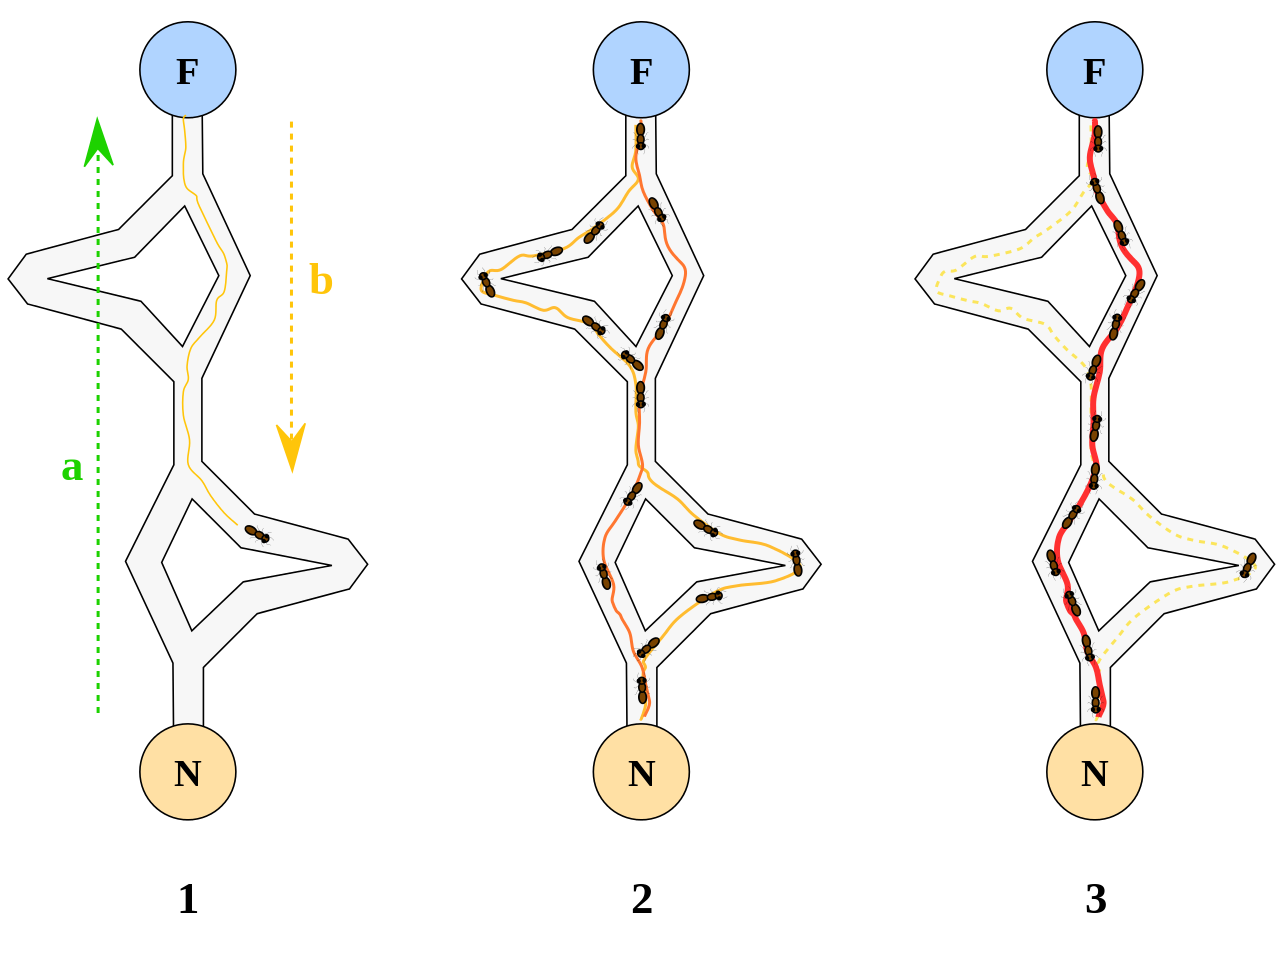
\includegraphics[width=0.7\textwidth]{ant.png}
		\caption{Работа муравьиной колонии}
		\label{ref:img1}}
\end{figure}

\begin{enumerate}
	\item первый муравей находит источник пищи (F) любым способом (а), а затем возвращается к гнезду (N), оставив за собой тропу из феромонов (b);
	\item затем муравьи выбирают один из четырёх возможных путей, затем укрепляют его и делают привлекательным;
	\item муравьи выбирают кратчайший маршрут, так как феромоны с более длинных путей быстрее испаряются.
\end{enumerate}

Вероятность перехода из вершины i в вершину j определяется по формуле \ref{form:way}.

\begin{equation}\label{form:way}
	p_{i,j}={\frac {(\tau_{i,j}^{\alpha })(\eta_{i,j}^{\beta })}{\sum (\tau_{i,j}^{\alpha })(\eta_{i,j}^{\beta })}}
\end{equation}

где $ \tau_{i,j} - $ расстояние от города i до j;

$\eta_{i,j} - $количество феромонов на ребре ij;

$\alpha - $ параметр влияния длины пути;

$\beta - $ параметр влияния феромона.

Уровень феромона обновляется в соответствии с формулой \ref{form:eva}


\begin{equation}\label{form:eva}
	\tau_{i,j}=(1-\rho )\tau_{i,j}+\Delta \tau_{i,j},
\end{equation}

где $\rho$ - \text{доля феромона, которая испарится;}

$\tau_{i,j}$ - \text{количество феромона на дуге ij;}

$\Delta \tau_{i,j}$ - количество отложенного феромона, вычисляется по формуле \ref{form:add1}.

\begin{equation}\label{form:add1}
	\Delta \tau_{i,j}= \tau_{i,j}^0 + \tau_{i,j}^1 + ... + \tau_{i,j}^k
\end{equation}

где k - количество муравьев в вершине графа с индексами i и j.


Описание поведения муравьев при выборе пути.

\begin{itemize}
	\item Муравьи имеют собственную «память».
	Поскольку каждый город может быть посещён только один раз, то у каждого муравья есть список уже посещенных городов - список запретов.
	Обозначим через $J_{ik}$ список городов, которые необходимо посетить муравью $k$, находящемуся в городе $i$.
	\item Муравьи обладают «зрением» - видимость есть эвристическое желание посетить город $j$ , если муравей находится в городе $i$.
	Будем считать, что видимость обратно пропорциональна расстоянию между городами.
	\item Муравьи обладают «обонянием» - они могут улавливать след феромона, подтверждающий желание посетить город $j$ из города $i$ на основании опыта других муравьёв.
	Количество феромона на ребре $(i,j)$ в момент времени $t$ обозначим через  $\tau_{i,j} (t)$.
	% \item На этом основании мы можем сформулировать вероятностно - пропорциональное правило, определяющее вероятность перехода $k$-ого муравья из города $i$  в город $j$.
	\item Пройдя ребро $(i,j)$ , муравей откладывает на нём некоторое количество феромона, которое должно быть связано с оптимальностью сделанного выбора.
	Пусть $T _{k} (t)$ есть маршрут, пройденный муравьем $k$ к моменту времени $t$ , $L _{k} (t)$ - длина этого маршрута, а $Q$ - параметр,
	имеющий значение порядка длины оптимального пути. Тогда откладываемое количество феромона может быть задано формулой \ref{form:add}.
	
\end{itemize}



\begin{equation}\label{form:add}
	{\displaystyle \Delta \tau_{i,j}^k={\begin{cases}Q/L_{k}, & {\mbox{если k-ый мурваей прошел по ребру ij;}}\\0,&{\mbox{иначе}}\end{cases}}}
\end{equation}

где Q - количество феромона, переносимого муравьем.

\section{Вывод}


В данном разделе были рассмотрены основополагающие материалы,
которые в дальнейшем потребуются при реализации алгоритмов для решения задачи коммивояжера.
